% EcoPath: condensed, author-review draft prepared from the supplied manuscript.
% Intended as an IEEE-style working version, NOT a claim of acceptance or publisher approval.
% Verify all numbers, model details, author identities, disclosure wording and source rights.
\documentclass[a4paper,conference,10pt]{IEEEtran}
\IEEEoverridecommandlockouts
\usepackage[T1]{fontenc}
\usepackage{amsmath,amssymb}
\usepackage{booktabs,tabularx,array,multirow}
\usepackage{graphicx}
\usepackage{xcolor}
\graphicspath{{figures/}}
\usepackage{url}
\usepackage{cite}
\usepackage{balance}
\usepackage[hidelinks]{hyperref}
\renewcommand{\arraystretch}{1.09}
\title{Evidence-Bounded Bird Conservation Report Drafting with QLoRA: A Matched Structured-Generation Study}
\author{\IEEEauthorblockN{Atharva Girkar, Taneesh Hinduja, Saransh Lulla, Ved Sarode, Indu Dokare}
\IEEEauthorblockA{Department of Computer Engineering, Vivekanand Education Society's Institute of Technology, Mumbai, India\\
\{2023.atharva.girkar, 2023.taneesh.hinduja, 2023.saransh.lulla, 2023.ved.sarode\}@ves.ac.in; indu.dokare@ves.ac.in}}
\begin{document}
\maketitle
\begin{abstract}
Conservation report drafting from incomplete biodiversity records requires explicit separation of supplied facts from unknowns. We study parameter-efficient adaptation of Qwen2.5-7B-Instruct for evidence-bounded drafting in EcoPath. An archived 15-species pilot found valid JSON in 15/15 adapted and 0/15 unadapted responses, under a prompt that did not explicitly require JSON. A separate matched study compares a newly trained QLoRA adapter with the unadapted model under identical engineered prompts and schema enforcement on 60 held-out species with three evidence variants (180 reports per condition). Under the prespecified punctuation-sensitive structured-field check, success was 1620/1620 for QLoRA and 1168/1620 for the unadapted model, a paired difference of 27.9 percentage points (95\% species-bootstrap interval: 27.2--29.0). A post-hoc analysis found that 435 of 443 assessable baseline value mismatches differed only by a terminal period. Ignoring terminal periods reduced the paired difference to 1.0 percentage point (95\% interval: 0.0--2.5). These are automated agreement measures for one evaluated seed and source format; they do not establish ecological correctness or conservation-decision validity.

\end{abstract}
\begin{IEEEkeywords}
QLoRA, biodiversity information, large language models, evidence grounding, structured generation
\end{IEEEkeywords}

\section{Introduction}
Conservation reports often combine reliable taxonomic metadata with incomplete evidence about species status, range, habitat, or threats. Large language models can produce fluent summaries, yet fluency need not imply that each statement is supported by the provided records. This distinction matters for citizen-science and aggregated biodiversity sources, where coverage and spatial bias affect interpretation \cite{ebird,gbifbias}. For human reviewers, a useful draft must retain known values and sources, mark absent evidence, and avoid presenting unverified assessments as facts.

EcoPath is a geospatial bird-intelligence platform whose report module organises selected species information into a structured draft. This paper concerns \emph{only that module}: image identification, map quality, ecological status prediction, and the wider platform's decision impact are outside the experiment. We investigate whether low-rank adaptation of an instruction-tuned language model improves schema-constrained reporting beyond a strongly prompted, unadapted counterpart. The questions are: (RQ1) does adaptation improve field-level agreement with supplied structured assertions under the same output contract, and (RQ2) does it preserve correct nulls when evidence is absent?

Our contributions are: (1) an evidence-availability evaluation with complete, partial, and minimal source variants; (2) a paired comparison that holds the prompt, constrained output schema, backbone, and test inputs fixed; and (3) separate reporting of available-value agreement, correct abstention, structural compliance, and limitations. An earlier taxonomy-only pilot is retained as historical context rather than pooled with the main evaluation. The overall EcoPath architecture is illustrated in Fig.~\ref{fig:architecture}.

% FIG. 1: Supplied PDF retained in figures/.
\begin{figure*}[!t]
\centering
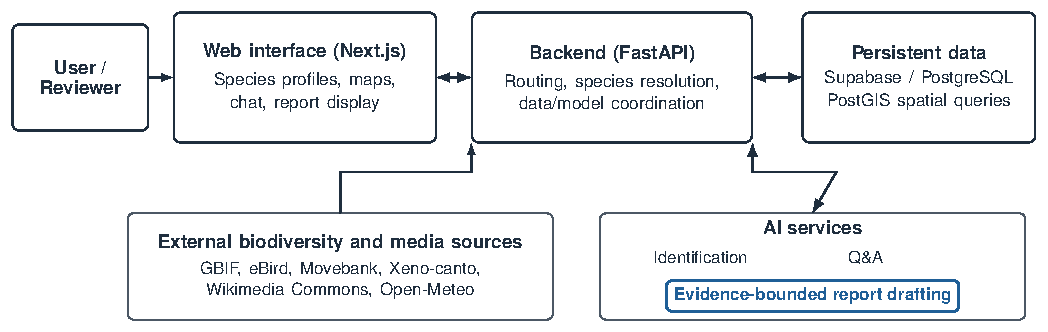
\includegraphics[width=\textwidth]{figure1_architecture.pdf}
\caption{EcoPath system architecture showing the Next.js interface, FastAPI backend, persistent data, external information sources, and AI services. The evidence-bounded report-drafting module is the experimental focus.}
\label{fig:architecture}
\end{figure*}

\section{Background and Related Work}
The eBird network provides substantial bird-observation data \cite{ebird}; GBIF aggregation introduces spatial-bias considerations \cite{gbifbias}. Machine learning for wildlife conservation requires ecological context and domain review \cite{tuia}. Prompt-based ecological information extraction has shown task-dependent capabilities \cite{castro}, and broader ecological question-answering benchmarks caution against treating language-model output as verified conservation expertise \cite{dorm,uryu}.

Retrieval-augmented generation can expose external evidence to the model \cite{rag}, but neither retrieval nor fluent citation alone proves that a generated value follows from a cited source. Output-format constraints similarly provide parseability without guaranteeing factual quality \cite{tam}. Low-rank adaptation (LoRA) updates compact trainable matrices \cite{lora}; QLoRA trains adapters with a quantised backbone \cite{qlora}. Hallucination studies \cite{ji} and documented biases in LLM-as-a-judge assessment \cite{zheng} motivate evaluating structured-value agreement directly rather than treating judge ratings as independent fact verification.

\section{Task and System Scope}
EcoPath combines a Next.js interface, a FastAPI orchestration layer, Supabase/PostgreSQL with PostGIS, and multiple biodiversity and media services. GBIF, eBird, Movebank, Xeno-canto, Wikimedia Commons, and Open-Meteo serve distinct platform functions. \emph{The experiment did not jointly test these services.} Its evaluated generator received curated species-linked assertions and source identifiers, not a complete environmental assessment. The separation between the wider platform and the evaluated drafting module is illustrated in Fig.~\ref{fig:architecture}.

The report contract was designed for nine evaluated fields per report: six fields potentially supported by the selected source material (recorded IUCN category, India-specific trend, habitat, range-size category, diet, migration) and three fields kept missing in the experimental records (population size, breeding, species-specific threats). A supported assertion should be copied with its expected source association; an unsupported field should be null. The output is a machine-readable draft for human review, not an IUCN Red List assessment.



\section{Experimental Method}
The matched evaluation pipeline is shown in Fig.~\ref{fig:pipeline}. Both inference arms receive identical evidence variants, prompting instructions, and output constraints; generated report drafts are evaluated only after generation.

% FIG. 2: Supplied PDF retained in figures/.
\begin{figure}[!t]
\centering
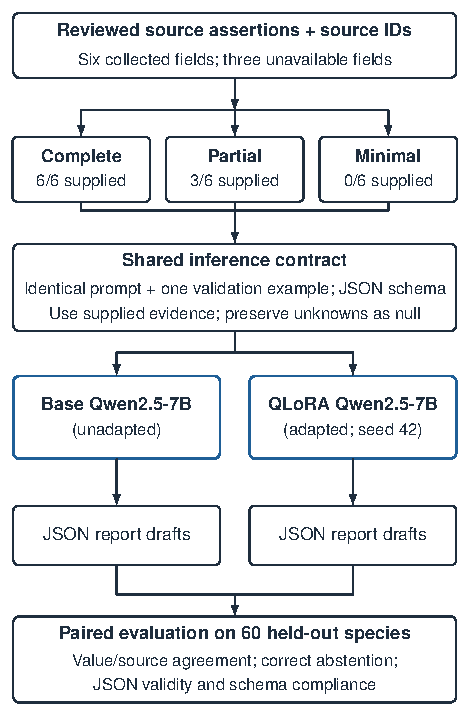
\includegraphics[width=\columnwidth]{figure2_pipeline.pdf}
\caption{Matched evidence-bounded report-drafting pipeline. Each species is evaluated with 6, 3, or 0 of the six collected fields supplied; both model conditions use the same prompt, demonstration, and schema constraint.}
\label{fig:pipeline}
\end{figure}

\subsection{Primary Dataset and Partitions}
We constructed an India-framed dataset of 120 species using a fixed \emph{State of India's Birds 2023} snapshot \cite{soib}. The source table contained 1,357 records, of which 942 were marked selected for SoIB; 44 exact scientific names in the historical dataset were excluded, leaving 898 candidates. A seed-42 round robin across current annual-trend categories selected 30 development species with distinct genera. From the remaining eligible names and genera, a second seed-9173 stratified round robin selected 90 species; the first 30 formed validation and the next 60 test. The resulting partitions have no shared genera and do not constitute a probability sample. Exact-name exclusion does not resolve all synonyms. Three names were updated using a later taxonomy crosswalk while stable source IDs remained anchored to the 2023 table. Source extraction was AI-assisted and checked against identified rows of the checksum-verified source, not independently validated by ornithologists.

For each species, \emph{complete}, \emph{partial}, and \emph{minimal} variants exposed six, three, and zero of the six collected fields, respectively. ``Complete'' refers to collected fields, not complete ecological evidence. For each species, seed 9173 and its stable species ID deterministically shuffled the six available fields; the partial variant masked three, and the minimal variant masked all six. A dependency check also masked direct echoes of hidden values; no additional dependency masks occurred in this dataset. Population size, breeding and species-specific threats remained absent in every variant. The resulting development and validation partitions each contained 90 examples, and the test partition contained 180 inputs per model. The split manifest and per-variant field masks are provided in the local supplement.

\begin{table}[t]
\centering
\caption{Test targets implied by the three evidence variants. Each row contains 60 reports with nine fields per report.}
\label{tab:availability}
\footnotesize
\begin{tabularx}{\columnwidth}{@{}>{\raggedright\arraybackslash}Xrrr@{}}
\toprule
\textbf{Variant} & \textbf{Known/ report} & \textbf{Non-null} & \textbf{Null}\\
\midrule
Complete & 6 & 360 & 180\\
Partial & 3 & 180 & 360\\
Minimal & 0 & 0 & 540\\
\midrule
Total (180 reports) & --- & 540 & 1080\\
\bottomrule
\end{tabularx}
\end{table}

Targets copied the provided values and source IDs and represented missing fields as null. This controls fidelity to the \emph{reviewed structured source assertions}; it does not supply independent truth labels for habitat, threat, or conservation status. The IUCN category, when present, is the category recorded in the archived source snapshot, not a claim about the current category or a replacement for India-specific conservation priority.

\subsection{Prompt and Output Contract}
Both arms used the same instruction to use supplied evidence only, return schema-conforming JSON, cite the supplied identifiers, and represent missing fields as null. The saved messages consist of a system message containing the complete JSON Schema, one validation user/assistant demonstration (\texttt{soib2023:Oenanthe\_fusca:partial}), and the test user message. The input serializes source values and synthetic canonical excerpts; original source-row excerpts and provenance remain in the local source ledger. A comparison of all 180 paired examples found identical message text, prompt token IDs, payload hashes, generation settings, and requested LM Format Enforcer constraints. The full verbatim messages, schema, native chat template, tokenizer IDs and example evidence are in the accompanying local supplement.

\subsection{Model Training and Matched Comparison}
The base model was Qwen2.5-7B-Instruct \cite{qwen} at pinned revision \texttt{a09a35458c702b33eeacc393d103063234e8bc28}. Both inference arms used a 4-bit NF4 backbone with double quantisation and FP16 computation. QLoRA used rank 16, $\alpha=32$, dropout 0.05, and adapters on \texttt{q\_proj}, \texttt{k\_proj}, \texttt{v\_proj}, \texttt{o\_proj}, \texttt{gate\_proj}, \texttt{up\_proj}, and \texttt{down\_proj}. The learning rate was $2\times10^{-4}$, batch size one, gradient accumulation eight, and training lasted three epochs (36 optimiser steps). Training used the native chat template, assistant-only loss, and no sequence truncation. Epoch checkpoints were selected by validation loss.

Three training seeds were run, but the matched test results in this paper evaluate \emph{only seed 42}, designated before either test arm was generated. The unadapted and adapted conditions received the same engineered prompt, one validation demonstration, an identical LM Format Enforcer schema constraint, greedy decoding, a 4096-token input budget, and up to 768 new tokens. No input evidence was truncated. Each arm attempted all 180 test variants in a separate process on an 8 GiB RTX 3070 Laptop GPU. The seed-42 adapter selected checkpoint 36 by minimum validation loss ($2.5038\times10^{-5}$); measured training time including validation and checkpoints was 1,304.9 s. The contrast isolates the tested adapter under the shared inference contract rather than comparing adaptation against a deliberately weak prompt.

\subsection{Outcome Definitions and Uncertainty}
The \emph{end-to-end field success} denominator includes nine expected fields for each of the 180 reports, totalling 1620 fields per arm. A field passes only if it contains the expected supplied value with its required source association, or the required null when evidence is absent. Fields of structurally invalid reports count as failures. For report $r$ and field $j$, success is defined by
\begin{equation}
\label{eq:criterion}
I_{rj}=\mathbf{1}[V_r\land M_{rj}\land C_{rj}],
\end{equation}
where $V_r$ denotes an assessable schema-valid, identity-matched, non-truncated output, $M_{rj}$ agreement with the expected value or null, and $C_{rj}$ the required source association (vacuously true for an absent value). Thus the primary rate is $\sum_{r,j}I_{rj}/1620$. String matching normalizes case and whitespace and maps explicit IUCN aliases, but preserves terminal punctuation; lists are compared without order. We separately report available-value agreement over 540 non-null targets, correct abstention over 1080 absent targets, schema compliance and source-associated agreement among assessable fields. A separately labeled post-hoc sensitivity analysis also removes terminal periods before applying the same comparison; it is not a semantic entailment test.

For uncertainty, the paired difference was calculated after averaging the three variants within each species; 2000 bootstrap resamples of species, keeping variants grouped, produced a percentile 95\% interval (bootstrap seed 42). This reflects test-species variation, \emph{not} variation across training seeds. We report exact counts to avoid interpreting error-free output on a finite test as a universal guarantee.

\section{Results}
\subsection{Primary Matched Evaluation}
Table~\ref{tab:main} reports the frozen strict check. Both conditions were almost always parseable under the shared schema constraint. The evaluated adapter matched 540/540 available targets and the unadapted model matched 94/540 under the punctuation-sensitive comparison. Correct null handling was already high in the unadapted condition (1074/1080). The numerical gap principally reflects exact serialization: 435 of 443 assessable baseline value mismatches differed only in a final period, and the other eight were shortened labels lacking the longer source-context phrase. These differences must not be interpreted as 443 demonstrated ecological errors.

\begin{table}[t]
\centering
\caption{Matched test results under the original punctuation-sensitive check: 60 species, 180 reports/arm.}
\label{tab:main}
\footnotesize
\begin{tabularx}{\columnwidth}{@{}>{\raggedright\arraybackslash}Xrr@{}}
\toprule
\textbf{Metric} & \textbf{Unadapted} & \textbf{QLoRA 42} \\
\midrule
Valid JSON & 179/180 & 180/180 \\
Full-schema compliance & 179/180 & 180/180 \\
End-to-end field success & 1168/1620 & 1620/1620 \\
Available-value agreement & 94/540 & 540/540 \\
Correct abstention & 1074/1080 & 1080/1080 \\
False abstention, assessable & 0/537 & 0/540 \\
Source-associated agreement & 94/537 & 540/540 \\
Generation-cap hits & 1 & 0 \\
Execution errors & 0 & 0 \\
\bottomrule
\end{tabularx}
\par\vspace{1mm}
\raggedright\scriptsize Strict matching preserves terminal periods. Source association is checked against reviewed structured assertions, not independent ecological truth. Structurally invalid or truncated reports count as failures.
\end{table}

The original end-to-end rates were 72.1\% (1168/1620) and 100.0\% (1620/1620), a paired difference of 27.9 percentage points (95\% species bootstrap: 27.2--29.0). In the post-hoc terminal-period-insensitive analysis, the corresponding counts were 1603/1620 and 1620/1620, a difference of 1.0 percentage point (95\% interval: 0.0--2.5); available-value agreement became 529/540 and 540/540. This sensitivity analysis was chosen after inspecting outputs and does not assess semantic equivalence. One unadapted report reached the generation cap, with no recorded execution errors.

\subsection{Sensitivity to Evidence Availability}
Under the punctuation-sensitive check, performance differed by evidence variant (Table~\ref{tab:variants}). The minimal case required nulls for every field and is therefore the least informative test of copying supplied values. The apparent baseline deficit with more evidence largely reflects terminal punctuation rather than demonstrated ecological errors. The evaluated adapter matched all structured-field checks in this sample, subject to the stated test limitations.

\begin{table}[t]
\centering
\caption{Punctuation-sensitive field success by evidence variant (540 fields per arm and variant).}
\label{tab:variants}
\footnotesize
\begin{tabularx}{\columnwidth}{@{}>{\raggedright\arraybackslash}Xrr@{}}
\toprule
\textbf{Input condition} & \textbf{Unadapted} & \textbf{QLoRA 42}\\
\midrule
Complete (6 supplied fields) & 240/540 (44.4\%) & 540/540 (100\%)\\
Partial (3 supplied fields) & 388/540 (71.9\%) & 540/540 (100\%)\\
Minimal (0 supplied fields) & 540/540 (100\%) & 540/540 (100\%)\\
\bottomrule
\end{tabularx}
\end{table}

The base arm's $0/537$ false-abstention count concerns only assessable fields expected to be non-null; it does not establish that those values matched exactly. The denominator is 537 rather than 540 because one partial-evidence output, \textit{Neophron percnopterus}, reached 768 output tokens and failed JSON parsing, excluding its three available fields from assessable-only rates. Its three available and six missing fields remain failures in end-to-end metrics. The matched adapted output was assessable. The output-source association metric also requires caution: matching a structured value and source ID does not establish that an unrestricted narrative claim is scientifically supported. Here, no claim-level human audit of generated prose was performed, and no formal ecological assessment was independently established.

\begin{table}[t]
\centering
\caption{A saved complete-evidence example illustrates a strict punctuation mismatch; both models cite the same source ID.}
\label{tab:example}
\footnotesize
\begin{tabularx}{\columnwidth}{@{}lX@{}}
\toprule
\textbf{Item} & \textbf{Saved value} \\
\midrule
Species / field & \textit{Hemipus picatus}, diet \\
Source excerpt & \texttt{Diet Guild=Invertebrate} (SoIB record 654) \\
Expected / QLoRA & \texttt{SoIB 2023 diet-guild classification: Invertebrate.} \\
Unadapted & \texttt{SoIB 2023 diet-guild classification: Invertebrate} \\
Source ID & \texttt{s-462f42e71095a56a34f3} \\
\bottomrule
\end{tabularx}
\end{table}

The example in Table~\ref{tab:example} is counted as a strict mismatch solely because the base output omits the last period. Another saved output for \textit{Acridotheres grandis} returned the diet value \texttt{Invertebrate} with the correct source ID but without the expected longer classification phrase; the adapted output retained that phrase. These are observed formatting/content differences, not independently adjudicated ecological errors. The local supplement contains full example inputs and outputs, including the truncated report.

\subsection{Historical Pilot and Illustrative Behavior}
Before the matched study, an archived QLoRA experiment trained on 85 synthetic taxonomy-only species reports and tested on 15 held-out species using a split seed of 42. The adapted model generated valid JSON with the six expected component keys in all 15 responses; the unadapted model generated Markdown prose in all 15. The pilot prompt, however, \emph{did not explicitly require JSON or supply the schema}, so this does not establish that tuning was necessary for structured output. Its data and adapter differ from the primary study; results are not pooled.

In two non-randomly selected pilot examples, Herring Gull and Common Murre, the unadapted report included threat descriptions not supported by the taxonomy-only input, whereas the adapter explicitly marked missing fields and retained the GBIF-linked source. The original automatic judge saw only a 600-character prefix of the prompt, generally excluding source excerpts; its format and grounding ratings are therefore omitted from the primary evidence table. These cases illustrate the value of explicit uncertainty statements, not a measured hallucination rate.

\section{Discussion}
\subsection{Interpretation and Alternative Explanations}
The matched design holds engineered prompts and schema enforcement constant. The baseline's 179/180 valid JSON outputs show that this format can largely be achieved without adaptation in the tested setting. The large strict-copying gap is predominantly attributable to omitted terminal periods; the smaller post-hoc punctuation-insensitive gap has an interval including zero. This study therefore does not establish a comparable gain in ecological fidelity. Both training targets and test inputs share a templated source representation, which favors assessment of structured copying rather than open-ended ecological reasoning.

\subsection{Threats to Validity}
However, the measured score is \emph{exact matching to reviewed assertions}, not conservation truth. First, source extraction was AI-assisted rather than independently adjudicated by ornithologists. Second, training and test examples came from the same construction approach, with only 120 non-randomly selected species; the no-overlapping-genera partition mitigates one form of leakage but cannot rule out shared template and source-distribution effects. Third, three adapters were trained but only the planned seed-42 adapter underwent matched testing; the bootstrap interval therefore cannot estimate training variability. Fourth, some ecological fields (notably population size, breeding, and species-specific threats) were never supplied, limiting conclusions about richer reports or real threat reasoning. Finally, no controlled user study measured reviewer time, trust, decision quality, or downstream conservation impact.

The single-GPU, batch-one mean wall times were 25.5\,s/report for the base condition and 29.4\,s/report for the adapter. They exclude model loading and one warm-up generation per arm and are not deployment throughput estimates. Seed-42 training used 1,304.9\,s including validation and checkpointing, excluding model loading and preprocessing. Extra latency and training cost must be weighed against task-specific fidelity; this study does not demonstrate a general cost advantage. The high adapted score could partly reflect the close match between supervised target patterns and the held-out structured contract. It does not establish robustness to free-form source passages, synonymic wording, inconsistent taxonomies, contradiction across evidence sources, or novel schema fields. Reviewer-facing deployment should preserve source excerpts, distinguish source claims from model statements, and support human correction before finalising any report. Future evaluations should replicate training seeds, include alternate non-fine-tuned controls, subject factual claims to independent specialist review, test distribution shifts and genuinely conflicting evidence, and study whether human reviewers make better decisions from the drafts.

\section{Reproducibility and Ethical Use}
The fixed 2023 State of India's Birds source \cite{soib}, source IDs, URLs, original row excerpts, retrieval dates, rights metadata, protocol, data hashes, adapter metadata, outputs and metric scripts are retained locally. The accompanying private supplement contains the exact matched messages and schema, split and mask manifests, paired outputs, metric audit, post-hoc sensitivity analysis and a reproduction guide. No public repository is claimed; reuse and redistribution terms for the newer taxonomy cross-check remain unresolved. The canonical JSON body of the frozen protocol, excluding its hash field, has SHA-256 \texttt{b0fc3242e40019a5\allowbreak 5578a50c2d10f866\allowbreak 3d4e5f0eab32a9bd\allowbreak c448270aea9e7d79}. This is distinct from the protocol file's byte-level SHA-256. The original seven-method, three-seed plan was reduced before these two matched test arms were generated; only seed 42 is evaluated here.

AI assistance was used in source-extraction review and manuscript preparation, and the archived pilot used teacher-generated targets and LLM-based historical ratings. Venue-specific disclosure requirements have not yet been selected. The system was not validated for autonomous conservation recommendations.

\section{Conclusion}
For evidence-bounded bird-report drafting in EcoPath, the seed-42 QLoRA adapter and a strongly prompted unadapted model were compared on 60 held-out species under identical schema constraints. The prespecified punctuation-sensitive check favored QLoRA by 27.9 percentage points, but 435 baseline mismatches differed only by a final period. A post-hoc punctuation-insensitive check reduced the paired difference to 1.0 percentage point, with a 95\% species-bootstrap interval of 0.0--2.5. These findings demonstrate sensitivity to output normalization and do not establish an ecological-fidelity advantage, cross-seed robustness, or practical conservation benefit. The historical pilot does not establish that fine-tuning is necessary for JSON generation.

\section*{Acknowledgment}
The authors acknowledge guidance from the Department of Computer Engineering, Vivekanand Education Society's Institute of Technology.

\begin{thebibliography}{14}\footnotesize
\bibitem{ebird} B. L. Sullivan \emph{et al.}, ``eBird: A citizen-based bird observation network in the biological sciences,'' \emph{Biological Conservation}, vol. 142, no. 10, pp. 2282--2292, 2009, doi: 10.1016/j.biocon.2009.05.006.
\bibitem{gbifbias} J. Beck, M. B\"oller, A. Erhardt, and W. Schwanghart, ``Spatial bias in the GBIF database and its effect on modeling species' geographic distributions,'' \emph{Ecological Informatics}, vol. 19, pp. 10--15, 2014, doi: 10.1016/j.ecoinf.2013.11.002.
\bibitem{rag} P. Lewis \emph{et al.}, ``Retrieval-augmented generation for knowledge-intensive NLP tasks,'' \emph{NeurIPS}, vol. 33, pp. 9459--9474, 2020.
\bibitem{lora} E. J. Hu \emph{et al.}, ``LoRA: Low-rank adaptation of large language models,'' \emph{ICLR}, 2022.
\bibitem{tuia} D. Tuia \emph{et al.}, ``Perspectives in machine learning for wildlife conservation,'' \emph{Nature Communications}, vol. 13, art. 792, 2022, doi: 10.1038/s41467-022-27980-y.
\bibitem{qlora} T. Dettmers, A. Pagnoni, A. Holtzman, and L. Zettlemoyer, ``QLoRA: Efficient finetuning of quantized LLMs,'' \emph{NeurIPS}, vol. 36, pp. 10088--10115, 2023.
\bibitem{ji} Z. Ji \emph{et al.}, ``Survey of hallucination in natural language generation,'' \emph{ACM Computing Surveys}, vol. 55, no. 12, art. 248, 2023, doi: 10.1145/3571730.
\bibitem{zheng} L. Zheng \emph{et al.}, ``Judging LLM-as-a-judge with MT-Bench and Chatbot Arena,'' \emph{NeurIPS}, vol. 36, 2023.
\bibitem{castro} A. Castro, J. Pinto, L. Reino, P. Pipek, and C. Capinha, ``Large language models overcome the challenges of unstructured text data in ecology,'' \emph{Ecological Informatics}, vol. 82, art. 102742, 2024, doi: 10.1016/j.ecoinf.2024.102742.
\bibitem{tam} Z. R. Tam \emph{et al.}, ``Let me speak freely? A study on the impact of format restrictions on large language model performance,'' in \emph{Proc. EMNLP Industry Track}, pp. 1218--1236, 2024, doi: 10.18653/v1/2024.emnlp-industry.91.
\bibitem{qwen} A. Yang \emph{et al.}, ``Qwen2.5 technical report,'' arXiv:2412.15115, 2024.
\bibitem{dorm} F. Dorm, J. Millard, D. Purves, M. Harfoot, and O. Mac Aodha, ``Large language models possess some ecological knowledge, but how much?'' \emph{Ecological Informatics}, vol. 95, art. 103699, 2026, doi: 10.1016/j.ecoinf.2026.103699.
\bibitem{uryu} S. Uryu, ``Evaluating large language models for IUCN Red List species information,'' arXiv:2510.02830, 2025.
\bibitem{soib} The SoIB Partnership, \emph{State of India's Birds: Range, Trends, and Conservation Status}, 2023 snapshot, Zenodo v1, doi: 10.5281/zenodo.11124590.
\end{thebibliography}
\end{document}
